\begin{center}
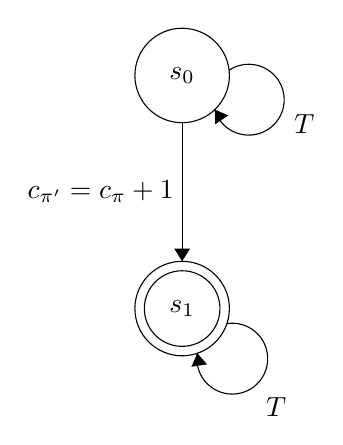
\begin{tikzpicture}[scale=0.2]
\tikzstyle{every node}+=[inner sep=0pt]
\draw [black] (35.2,-20.3) circle (3);
\draw (35.2,-20.3) node {$s_0$};
\draw [black] (35.2,-35.1) circle (3);
\draw (35.2,-35.1) node {$s_1$};
\draw [black] (35.2,-35.1) circle (2.4);
\draw [black] (38.03,-36.06) arc (99:-189:2.25);
\draw (40.5,-41.35) node [right] {$T$};
\fill [black] (36.16,-37.93) -- (35.79,-38.8) -- (36.78,-38.64);
\draw [black] (38.17,-19.973) arc (124.01689:-163.98311:2.25);
\draw (42.3,-23.39) node [right] {$T$};
\fill [black] (37.27,-22.46) -- (37.3,-23.4) -- (38.13,-22.84);
\draw [black] (35.2,-23.3) -- (35.2,-32.1);
\fill [black] (35.2,-32.1) -- (35.7,-31.3) -- (34.7,-31.3);
\draw (34.7,-27.7) node [left] {$c_{\pi'}=c_\pi+1$};
\end{tikzpicture}
\end{center}